\documentclass[12pt,a4paper]{article}

% ---------------------------------------------------
% GRUNDSPRACHE & SCHRIFT
% ---------------------------------------------------
\usepackage[ngerman]{babel}
\usepackage{fontspec}
\setmainfont{Times New Roman}

% ---------------------------------------------------
% SEITENLAYOUT
% ---------------------------------------------------
\usepackage{geometry}
\geometry{
    left=4cm,
    right=2cm,
    top=4cm,
    bottom=2cm,
    headsep=20pt
}

% ---------------------------------------------------
% FORMATIERUNG
% ---------------------------------------------------
\usepackage{setspace}
\onehalfspacing

\setlength{\parskip}{6pt}
\setlength{\parindent}{0pt}

\usepackage{ragged2e}
\justifying

% automatische Silbentrennung aktiv lassen
\pretolerance=100
\tolerance=2000
\emergencystretch=1em

% ---------------------------------------------------
% ÜBERSCHRIFTEN
% ---------------------------------------------------
\usepackage{titlesec}

\titleformat{\section}
  {\normalfont\bfseries\fontsize{12}{14}\selectfont}
  {\thesection}{1em}{}

\titleformat{\subsection}
  {\normalfont\bfseries\fontsize{12}{14}\selectfont}
  {\thesubsection}{1em}{}

\titleformat{\subsubsection}
  {\normalfont\bfseries\fontsize{12}{14}\selectfont}
  {\thesubsubsection}{1em}{}

\titlespacing*{\section}{0pt}{12pt}{6pt}
\titlespacing*{\subsection}{0pt}{12pt}{6pt}
\titlespacing*{\subsubsection}{0pt}{12pt}{6pt}

% Jedes Hauptkapitel auf neuer Seite
\usepackage{etoolbox}
\pretocmd{\section}{\clearpage}{}{}

% ---------------------------------------------------
% GRAFIKEN, TABELLEN, MATHE
% ---------------------------------------------------
\usepackage{graphicx}
\graphicspath{{../Screenshots/}}
\usepackage{booktabs}
\usepackage{amsmath}
\usepackage{caption}

\captionsetup{
    font=normalsize,
    labelfont=bf,
    justification=raggedright,
    singlelinecheck=false,
    skip=6pt
}

% Tabellen- und Abbildungsüberschriften oben
\captionsetup[table]{position=top}
\captionsetup[figure]{position=top}
\newcommand{\figsource}{\caption*{\footnotesize Quelle: Eigene Darstellung}}

% ---------------------------------------------------
% CODE
% ---------------------------------------------------
\usepackage{listings}
\renewcommand{\lstlistlistingname}{Codeverzeichnis}

\lstset{
    basicstyle=\ttfamily\small,
    breaklines=true,
    frame=single,
    captionpos=t,
    numbers=left,
    numberstyle=\tiny,
    numbersep=8pt
}

% ---------------------------------------------------
% ZITATE, LINKS, VERZEICHNISSE
% ---------------------------------------------------
\usepackage{csquotes}
\usepackage[nottoc]{tocbibind}
\usepackage{tocloft}
\usepackage[hidelinks]{hyperref}

% Inhaltsverzeichnis nur bis Ebene 2 anzeigen:
% section und subsection, also z. B. 1 und 1.1
\setcounter{tocdepth}{2}

% Bezeichnung
\renewcommand{\contentsname}{Inhaltsverzeichnis}

% Überschrift des Inhaltsverzeichnisses wie im FOM-Beispiel:
% linksbündig, fett, 12 pt
\renewcommand{\cfttoctitlefont}{\normalfont\bfseries\fontsize{12}{14}\selectfont}
\renewcommand{\cftaftertoctitle}{\par\vspace{12pt}}
\setlength{\cftbeforetoctitleskip}{0pt}
\setlength{\cftaftertoctitleskip}{12pt}

% Überschriften von Abbildungs- und Tabellenverzeichnis ebenfalls 12 pt fett
\renewcommand{\cftloftitlefont}{\normalfont\bfseries\fontsize{12}{14}\selectfont}
\renewcommand{\cftlottitlefont}{\normalfont\bfseries\fontsize{12}{14}\selectfont}
\setlength{\cftbeforeloftitleskip}{0pt}
\setlength{\cftbeforelottitleskip}{0pt}
\setlength{\cftafterloftitleskip}{12pt}
\setlength{\cftafterlottitleskip}{12pt}

% Schrift der Einträge im Inhaltsverzeichnis:
% normal, nicht fett
\renewcommand{\cftsecfont}{\normalfont}
\renewcommand{\cftsecpagefont}{\normalfont}

\renewcommand{\cftsubsecfont}{\normalfont}
\renewcommand{\cftsubsecpagefont}{\normalfont}

\renewcommand{\cftsubsubsecfont}{\normalfont}
\renewcommand{\cftsubsubsecpagefont}{\normalfont}

% ---------------------------------------------------
% Punktlinien direkt wie: Eintrag........................................7
% ---------------------------------------------------
\makeatletter

% Sehr enge Punktreihe ohne Zusatzabstände
\newcommand{\tocdirectdots}{%
  \nobreak
  \leaders\hbox{.}\hfill
  \nobreak
}

% Punktreihen im Inhaltsverzeichnis
\renewcommand{\cftsecleader}{\tocdirectdots}
\renewcommand{\cftsubsecleader}{\tocdirectdots}
\renewcommand{\cftsubsubsecleader}{\tocdirectdots}

% Punktreihen im Abbildungs- und Tabellenverzeichnis
\renewcommand{\cftfigleader}{\tocdirectdots}
\renewcommand{\cfttableader}{\tocdirectdots}

% Seitenzahlen ohne feste Box direkt hinter den Punkten
\renewcommand{\cftsecfillnum}[1]{%
  {\cftsecleader}{\cftsecpagefont #1}\cftsecafterpnum\par
}

\renewcommand{\cftsubsecfillnum}[1]{%
  {\cftsubsecleader}{\cftsubsecpagefont #1}\cftsubsecafterpnum\par
}

\renewcommand{\cftsubsubsecfillnum}[1]{%
  {\cftsubsubsecleader}{\cftsubsubsecpagefont #1}\cftsubsubsecafterpnum\par
}

\renewcommand{\cftfigfillnum}[1]{%
  {\cftfigleader}{\cftfigpagefont #1}\cftfigafterpnum\par
}

\renewcommand{\cfttabfillnum}[1]{%
  {\cfttableader}{\cfttabpagefont #1}\cfttabafterpnum\par
}

\makeatother

% rechter Rand für Seitenzahlen
\cftsetpnumwidth{0pt}
\cftsetrmarg{0pt}

% Einzüge wie im FOM-Beispiel
\setlength{\cftsecindent}{0pt}
\setlength{\cftsubsecindent}{1.5em}
\setlength{\cftsubsubsecindent}{3.0em}

% Breite der Nummernspalten
\setlength{\cftsecnumwidth}{2.2em}
\setlength{\cftsubsecnumwidth}{2.8em}
\setlength{\cftsubsubsecnumwidth}{3.4em}

% Abstand zwischen den Einträgen im Inhaltsverzeichnis
\setlength{\cftbeforesecskip}{6pt}
\setlength{\cftbeforesubsecskip}{3pt}
\setlength{\cftbeforesubsubsecskip}{3pt}
\setlength{\cftparskip}{0pt}

% ---------------------------------------------------
% KOPF-/FUSSZEILEN
% ---------------------------------------------------
\usepackage{fancyhdr}
\pagestyle{fancy}
\fancyhf{}
\renewcommand{\headrulewidth}{0pt}
\fancyhead[C]{\thepage}
\setlength{\headheight}{15pt}

% Seitenzahlen auch auf Verzeichnisseiten oben
\renewcommand{\headrulewidth}{0pt}
\fancypagestyle{plain}{%
  \fancyhf{}
  \fancyhead[C]{\thepage}
}

% ---------------------------------------------------
% LITERATUR
% ---------------------------------------------------
\usepackage[
backend=biber,
style=authoryear,
autocite=footnote,
sorting=nyt,
maxcitenames=2,
maxbibnames=99,
giveninits=true,
uniquename=false,
uniquelist=false,
doi=false,
isbn=false,
url=true
]{biblatex}

\addbibresource{literatur.bib}

\DefineBibliographyStrings{ngerman}{
  andothers = {et al.},
  page = {S.},
  pages = {S.}
}

\renewcommand*{\postnotedelim}{\addcomma\space}

% ---------------------------------------------------
% DOKUMENTBEGINN
% ---------------------------------------------------
\begin{document}

% ---------------------------------------------------
% TITELBLATT
% ---------------------------------------------------
\begin{titlepage}
\begin{center}

    
\includegraphics[width=4cm]{FOM_Logo01_2012_rgb.jpg} \\[0.5cm]

    \textbf{FOM Hochschule für Oekonomie \& Management} \\
    Hochschulzentrum Bonn \\[1.0cm]

    {\Large Berufsbegleitender Studiengang Wirtschaftsinformatik} \\[0.2cm]
    zum \\[0.2cm]
    Bachelor of Science (B.Sc.) \\[0.2cm]
    6. Semester \\[1.5cm]

    Seminararbeit im Modul ERP-Systeme zum Thema \\[1.0cm]

    {\Large\textbf{End-to-End-Automatisierung von Produkt- und Lagerprozessen in Odoo}} \\[1.5cm]

\end{center}

\vfill

\begin{flushleft}
\begin{tabular}{@{}ll@{}}
Dozent: & Dipl. Ing. Sandro Coletta \\
Name: & Lorenz Chylka, Leonard Reglin \\
Matrikelnummer: & 736986, 740270 \\
Studiengang: & Wirtschaftsinformatik \\
Semester: & 6. Semester \\
Abgabedatum: & TT.MM.JJJJ \\
Wörter Hausarbeit: & XXX \\
Wörter Code: & XXX \\
\end{tabular}
\end{flushleft}

\end{titlepage}

% ---------------------------------------------------
% VERZEICHNISSE: RÖMISCHE SEITENZAHLEN
% ---------------------------------------------------
\pagenumbering{Roman}
\setcounter{page}{2}

\tableofcontents
\newpage

\listoffigures
\section*{KI-Nutzung}
\addcontentsline{toc}{section}{KI-Nutzung}

In dieser wissenschaftlichen Arbeit wurden zur sprachlichen Unterstützung bei der Erstellung des Textes KI-Modelle eingesetzt. Insbesondere wurden ChatGPT und DeepL zur Verbesserung der Grammatik, Struktur, Rechtschreibung und Lesbarkeit verwendet. Die inhaltliche Konzeption, Argumentation und jedwede Schlussfolgerungen liegen jedoch vollständig in der Verantwortung des Autors. Sollten Fremdwerke verwendet worden sein, sind diese entsprechend durch Fußnoten gekennzeichnet.

\section*{Geschlechterinklusive Sprache} 
\addcontentsline{toc}{section}{Geschlechterinklusive Sprache}
In diesem Text wird aus Gründen der Lesbarkeit und Tradition häufig die maskuline Form verwendet. Dennoch sei betont, dass sich alle Ausführungen und Bezeichnungen geschlechtsübergreifend auf Personen aller Geschlechteridentitäten beziehen. Die Wahl der sprachlichen Form soll in keinem Fall als Ausschluss oder Diskriminierung anderer Geschlechter verstanden werden.
\newpage

\listoftables
\newpage

\section*{Abkürzungsverzeichnis}
\addcontentsline{toc}{section}{Abkürzungsverzeichnis}

\begin{tabular}{@{}ll@{}}
API & Application Programming Interface \\
EAN & European Article Number \\
ERP & Enterprise Resource Planning \\
GTIN & Global Trade Item Number \\
IT & Informationstechnologie \\
KI & Künstliche Intelligenz \\
REST & Representational State Transfer \\
\end{tabular}

% ---------------------------------------------------
% TEXTTEIL: ARABISCHE SEITENZAHLEN
% ---------------------------------------------------
\newpage
\pagenumbering{arabic}
\setcounter{page}{1}

\section{Einleitung}

Die fortschreitende Digitalisierung von betrieblichen Wertschöpfungsprozessen führt dazu, dass Unternehmen in zunehmendem Maße auf integrierte ERP-Systeme (Enterprise Resource Planning) angewiesen sind. Diese werden genutzt. um Datenkonsistenz, Prozessqualität und operative Effizienz sicherzustellen. Besonders im Einzelhandel und in der Lebensmittelbranche besteht ein hoher Bedarf an aktuellen, strukturierten und fehlerfreien Produktstammdaten, da diese unmittelbar Grundlage für logistische, kaufmännische und kundenbezogene Prozesse und Entscheidungen sind. \autocite[Vgl.][]{krcmar2022}

Für kleine und mittlere Unternehmen stellt die manuelle Pflege dieser Stammdaten jedoch eine erhebliche Belastung dar. Uneinheitliche Datenquellen, redundante Datenerfassungen und fehlende Standardisierung führen zu inkonsistenten Datensätzen, Medienbrüchen und betrieblichen Ineffizienzen. \autocite[Vgl.][]{gronau2017} Da fehlerhafte oder unvollständige Stammdaten unmittelbare Auswirkungen auf Lagerprozesse, Verkaufsabläufe und betriebliche Entscheidungen haben, gilt das Stammdatenmanagement als ein kritischer Erfolgsfaktor für ERP-basierte Prozessautomatisierung. Hochwertige Daten bilden die Voraussetzung dafür, dass ERP-Systeme wie Odoo zuverlässig arbeiten und automatisierte Prozesse korrekt ausgeführt werden können \autocite[Vgl.][]{lausen2020}.

ERP-Systeme ermöglichen dabei die integrierte Abbildung zentraler Unternehmensprozesse und stellen eine einheitliche Datenbasis für verschiedene Funktionsbereiche bereit. Durch die zentrale Speicherung und Verarbeitung von Informationen können Redundanzen reduziert und Transparenz innerhalb der Organisation erhöht werden. \autocite[vgl.][]{davenport1998} Insbesondere im Bereich des Bestands- und Lagermanagements, sowie im Stammdatenmanagement tragen ERP-Systeme dazu bei, die Genauigkeit von Inventardaten zu verbessern und operative Abläufe effizienter zu gestalten. \autocite[vgl.][]{romney2018}

Darüber hinaus ermöglichen ERP-Systeme eine Echtzeitverarbeitung von Daten und fördern die bereichsübergreifende Zusammenarbeit innerhalb der Supply Chain. Studien zeigen, dass der Einsatz von ERP-Systemen signifikant zur Verbesserung der operativen Effizienz beitragen kann, da Prozesse besser koordiniert und Informationsflüsse optimiert werden können. \autocite[vgl.][]{chopra2016} Insbesondere durch die Automatisierung wiederkehrender Aufgaben und die Integration verschiedener Unternehmensbereiche können Fehlerquellen reduziert und Entscheidungsprozesse beschleunigt werden. \autocite[vgl.][]{chang2014}

In der Lagerlogistik spielt die Qualität der Produktstammdaten eine zentrale Rolle. Fehlende oder inkonsistente Daten führen häufig zu falschen Bestandsbuchungen, ineffizienten Auftragsabwicklungen und erhöhten Kosten entlang der gesamten Lieferkette. Moderne ERP-Systeme ermöglichen eine präzisere Steuerung von Beständen und eine bessere Nachverfolgbarkeit von Warenströmen. \autocite[vgl.][]{chopra2016}

Gleichzeitig steigt die Bedeutung externer Datenquellen für die Anreicherung von Produktinformationen. Offene Datenbanken wie Open Food Facts stellen strukturierte und maschinenlesbare Produktdaten bereit, die über standardisierte Schnittstellen, sogenannte API's (Application Programming Interface), abgerufen werden können. Diese Entwicklung eröffnet neue Möglichkeiten zur Automatisierung der Stammdatenpflege und zur Reduktion manueller Eingaben, wodurch sowohl die Datenqualität als auch die Prozesseffizienz nachhaltig verbessert werden können.

\subsection{Problemstellung}

Im Lebensmitteleinzelhandel müssen Produktstammdaten wie Produktbezeichnungen, Herstellerinformationen, Zutatenlisten, Allergenkennzeichnungen, Nährwerttabellen sowie EAN- und GTIN-Barcodes (EAN: European Article Number; GTIN: Global Trade Item Number) kontinuierlich aktualisiert werden, da sie die Grundlage für zahlreiche betriebliche Prozesse bilden. Die manuelle Erfassung dieser Informationen ist jedoch zeitintensiv, fehleranfällig und bindet erhebliche personelle Ressourcen. In der Praxis führt dies häufig zu inkonsistenten oder unvollständigen Datensätzen, redundanten Datenbeständen in unterschiedlichen Systemen sowie zu Übertragungsfehlern bei der Pflege und Aktualisierung der Informationen.

Wissenschaftliche Untersuchungen zeigen, dass eine unzureichende Datenqualität in ERP-Systemen maßgeblich zu ineffizienten Geschäftsprozessen, Fehlentscheidungen und erhöhten Prozesskosten beiträgt, was die steigende Relevanz eines strukturierten und qualitativ hochwertigen Stammdatenmanagements unterstreicht \autocite[Vgl.][]{gronau2017} (vgl. Niedermeier, 2025;)ACHTUNG. Gleichzeitig bieten offene Produktdatenbanken wie Open Food Facts standardisierte, strukturierte und maschinenlesbare Produktinformationen, die einen geeigneten Ansatzpunkt für die Automatisierung der Stammdatenpflege darstellen und dadurch das Potenzial besitzen, die Qualität und Aktualität von Produktdaten erheblich zu verbessern.

\subsection{Zielsetzung der Arbeit}

Ziel der vorliegenden Arbeit ist die Konzeption und prototypische Umsetzung einer End-to-End-Systemarchitektur, die eine automatisierte Produkt- und Lagerdatenverarbeitung in Odoo ermöglicht. Der entwickelte Prototyp soll demonstrieren, wie Barcode-Erfassung, API-basierte Datenanreicherung und darauf aufbauende ERP-Prozesse technisch miteinander verknüpft werden können, um die Qualität von Produktstammdaten zu verbessern.

Im Mittelpunkt steht dabei die Erfassung von Barcodes über geeignete Eingabegeräte, der anschließende Abruf und Vervollständigung der Produktdaten über die Open-Food-Facts-API sowie die darauf basierende Erstellung oder Aktualisierung eines Produktstammsatzes innerhalb von Odoo. Darüber hinaus soll gezeigt werden, wie die angereicherten Daten in die Lagerprozesse des Inventory-Moduls integriert werden können und wie sie nachgelagerte Verkaufsprozesse im Sales-Modul unterstützen.

Die Arbeit untersucht insgesamt, in welchem Ausmaß der Einsatz externer Datenquellen und teilautomatisierter Informationsflüsse dazu beiträgt, die Qualität des Stammdatenbestands zu erhöhen und zugleich die Prozesskosten in den Bereichen Produktanlage, Lagerverwaltung und Verkauf nachhaltig zu reduzieren.

\section{Grundlagen}

Dieses Kapitel stellt zentrale Fachbegriffe und technologische Grundlagen bereit, die für die spätere Analyse und Implementierung erforderlich sind (vgl. Theisen, 2021, S. 136) QUELLE.

\subsection{ERP-Systeme und Produktstammdaten}

ERP-Systeme ermöglichen die integrierte Abbildung von Geschäftsprozessen und die zentrale Verwaltung betrieblicher Daten. Odoo ist ein modulares Open-Source-ERP-System mit integrierter PostgreSQL-Datenbank und über 30 Standardmodulen.

Relevante Module für die vorliegende Arbeit sind:

\begin{itemize}
    \item \textbf{Inventory (Lagerverwaltung)} -- Verwaltung von Beständen und Lagerbewegungen.
    \item \textbf{Sales (Vertrieb)} -- Auftragsabwicklung und Versandprozesse.
    \item \textbf{Purchase (Einkauf)} -- Bestell- und Beschaffungsprozesse.
    \item \textbf{Barcode-Modul} -- Eigen erstelltes Modul zur Verarbeitung gescannter Barcodes und Aktionen in Odoo.
\end{itemize}

\subsection{Barcodes und Produktidentifikation}

Barcodes, beispielsweise EAN-13, sind standardisierte maschinenlesbare Produktkennzeichen. In der Lagerlogistik verbessern sie die Identifikation von Artikeln, die Beschleunigung von Wareneingang und Inventur sowie die Reduktion manueller Fehler.

\subsection{Schnittstellen und Open-Food-Facts-API}

Open Food Facts ist eine offene, kollaborative Lebensmitteldatenbank. Die Produktinformationen werden über eine öffentlich zugängliche REST-API bereitgestellt. Der API-Endpunkt für Barcodes lautet:

\begin{lstlisting}[caption={API-Endpunkt für Produktabfragen über Barcode}]
https://world.openfoodfacts.org/api/v0/product/{barcode}.json
\end{lstlisting}

Die API liefert unter anderem Produktnamen, Zutaten und Allergene, Nährwerttabellen, Marken, Kategorien sowie Produktbilder.

\section{Konzeption und Umsetzung des Barcode-API-Submoduls}

Dieses Kapitel beschreibt funktionale und nichtfunktionale Anforderungen, die als Grundlage für die Implementierung dienen.


\subsection{Anforderungen an das Submodul}

\begin{itemize}
    \item Erfassung eines Barcodes über ein Endgerät.
    \item Abfrage der Produktdaten über die Open-Food-Facts-API.
    \item Automatische Erstellung oder Aktualisierung eines Produkts in Odoo.
    \item Zuordnung des Artikels zum Lagerbestand.
    \item Unterstützung des Verkaufsprozesses im Sales-Modul.
\end{itemize}

\subsection{Nichtfunktionale Anforderungen}

\begin{itemize}
    \item Performante Verarbeitung von API-Antworten.
    \item Fehlertoleranz bei nicht bekannten Barcodes.
    \item Erweiterbarkeit für weitere Datenquellen.
    \item Konsistente Datenhaltung im ERP-System.
\end{itemize}

\section{Odoo als Systembasis}

Odoo bildet die technische Systembasis des entwickelten Prototyps, da zentrale Produkt-, Lager- und Verkaufsprozesse innerhalb einer integrierten ERP-Umgebung abgebildet werden können. Das System ist modular aufgebaut und stellt unterschiedliche Anwendungen bereit, die auf einer gemeinsamen Datenbasis miteinander verbunden werden. Für die vorliegende Arbeit sind insbesondere die Produktverwaltung, die Lagerverwaltung sowie die technische Erweiterbarkeit durch individuell entwickelte Module relevant.

Die im Prototyp verwendete Barcode-Funktionalität basiert nicht auf dem von Odoo standardmäßig bereitgestellten Barcode-Modul. Stattdessen wird ein eigenständig programmiertes Custom-Submodul eingesetzt, das Barcodes entgegennimmt, externe Produktdaten über die Open-Food-Facts-API abruft und diese Daten anschließend in die Produkt- und Lagerstrukturen von Odoo überführt. Odoo wird damit nicht als vollständige Standardlösung verwendet, sondern als ERP-Systembasis, die durch eine projektspezifische Erweiterung an den vorliegenden Anwendungsfall angepasst wird.


\subsection{Produkt- und Lagerverwaltung in Odoo}

Die Produktverwaltung in Odoo erfolgt über zentrale Produktmodelle, in denen grundlegende Produktstammdaten wie Produktbezeichnung, Verkaufspreis, Kategorie und Barcode gespeichert werden können. Dabei wird zwischen Produktvorlagen und konkreten Produktvarianten unterschieden. Produktvorlagen dienen der Verwaltung allgemeiner Produktinformationen, während Produktvarianten spezifische Ausprägungen eines Produkts abbilden können.\autocite{odoo2026productmanagement}

Abbildung \ref{fig:produkt-uebersicht} zeigt die Produktübersicht im Prototyp, während Abbildung \ref{fig:produkt-vendor} die Verknüpfung eines Produkts mit einem Lieferanten dokumentiert. Beide Ansichten sind für die spätere automatische Produktanlage und die Beschaffungslogik relevant.

\begin{figure}[htbp]
  \centering
  \caption{Produktübersicht im Odoo-Prototyp}
  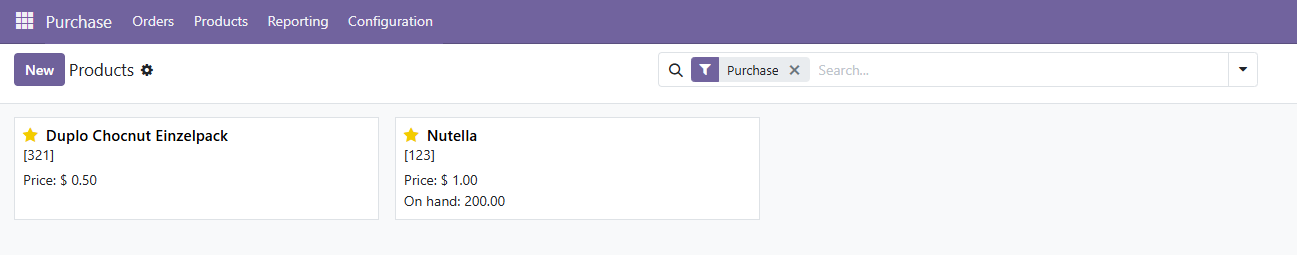
\includegraphics[width=0.95\textwidth]{Produkt Übersicht.png}
  \figsource
  \label{fig:produkt-uebersicht}
\end{figure}

\begin{figure}[htbp]
  \centering
  \caption{Verknüpfung eines Produkts mit einem Lieferanten}
  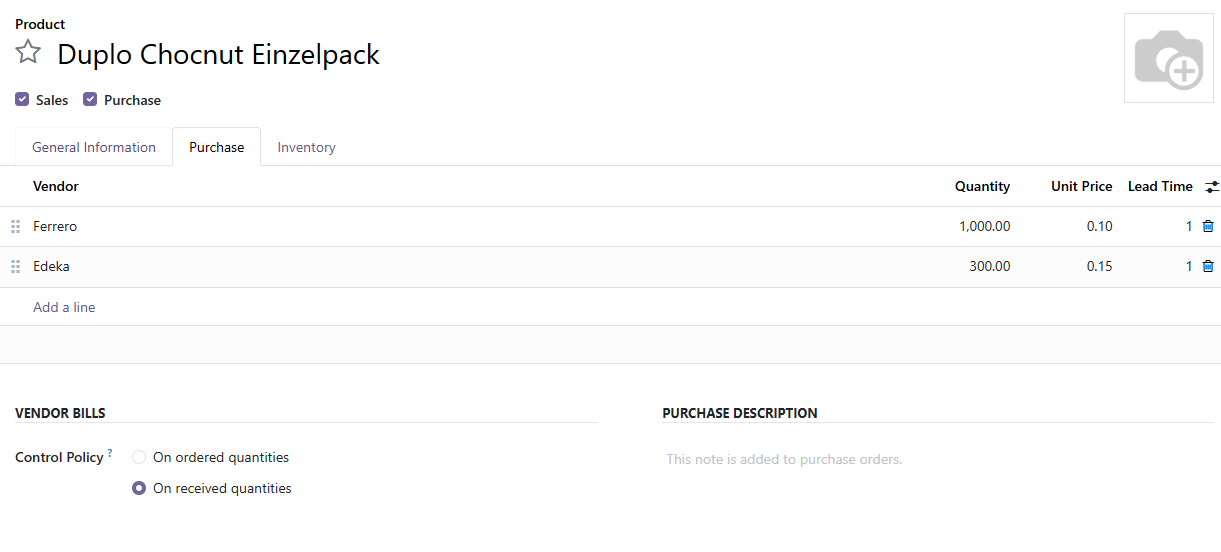
\includegraphics[width=0.95\textwidth]{Produkt mit Vendor Verknüpfen.png}
  \figsource
  \label{fig:produkt-vendor}
\end{figure}

Für die Lagerverwaltung stellt Odoo das Inventory-Modul bereit. Dieses ermöglicht die Verwaltung von Lagerorten, Beständen, Wareneingängen, internen Umlagerungen und Warenausgängen. Lagerbewegungen werden systemseitig dokumentiert und mit den entsprechenden Produkten verknüpft. Dadurch können Bestände nicht isoliert, sondern im Zusammenhang mit den zugrunde liegenden Produktstammdaten verarbeitet werden.\autocite{odoo2026inventory}
Im Kontext der vorliegenden Arbeit ist diese Verbindung zwischen Produkt- und Lagerverwaltung wesentlich. Ein Produkt, das durch das Custom-Submodul automatisch angelegt oder aktualisiert wird, kann anschließend unmittelbar in lagerbezogene Prozesse eingebunden werden. Dazu zählen beispielsweise die Zuordnung zu einem Lagerbestand, die spätere Verbuchung von Wareneingängen oder die Verwendung in Verkaufsprozessen. Die Produktdaten dienen somit als Stammdatenbasis für nachgelagerte ERP-Prozesse.

Die Verwendung von Barcodes unterstützt dabei die eindeutige Identifikation von Produkten. In Odoo können Barcodes als Bestandteil der Produktstammdaten gespeichert werden. Dadurch kann ein gescannter Code einem bestehenden Produktdatensatz zugeordnet werden. Für den entwickelten Prototyp wird diese Möglichkeit genutzt, jedoch nicht über das standardmäßige Odoo-Barcode-Modul umgesetzt. Der Barcode wird vielmehr durch ein eigenes Submodul verarbeitet, das die Produktidentifikation mit einer externen Datenabfrage verbindet. \autocite{odoo2026productmanagement}

Zur Umsetzung der automatisierten Produktanlage wird Odoo durch ein eigenständig entwickeltes Custom-Submodul erweitert. Dieses Submodul ist nicht mit dem von Odoo bereitgestellten Barcode-Modul gleichzusetzen. Es handelt sich um eine projektspezifische Erweiterung, die ausschließlich für den in dieser Arbeit betrachteten Prozess entwickelt wird. Die Aufgabe des Submoduls besteht darin, einen eingegebenen oder gescannten Barcode zu verarbeiten, eine Anfrage an die Open-Food-Facts-API zu stellen und die zurückgegebenen Produktinformationen in Odoo weiterzuverarbeiten.

Die technische Erweiterbarkeit von Odoo wird durch das modulare Entwicklungsmodell ermöglicht. Ein Odoo-Modul besteht typischerweise aus einer Manifest-Datei, Python-Dateien für die Geschäftslogik sowie XML-Dateien zur Definition von Ansichten, Menüs und weiteren Konfigurationen.\autocite{odoo2026orm} Die Geschäftslogik wird über Python-Klassen umgesetzt, die auf das Object-Relational-Mapping von Odoo zugreifen. Dadurch können bestehende Datenmodelle erweitert oder neue Modelle definiert werden.\autocite{odoo2026orm}

Das entwickelte Custom-Submodul wird zwischen Barcode-Erfassung, externer API-Abfrage und Produktverwaltung positioniert. Nach Eingabe eines Barcodes wird zunächst geprüft, ob in Odoo bereits ein Produkt mit diesem Barcode existiert. Falls ein entsprechender Datensatz vorhanden ist, können die vorhandenen Informationen aktualisiert oder ergänzt werden. Falls kein Produkt gefunden wird, wird ein neuer Produktstammsatz angelegt. Die über die Open-Food-Facts-API abgerufenen Daten werden dabei auf die relevanten Felder des Odoo-Produktmodells abgebildet. Hierzu zählen insbesondere Produktname, Marke, Barcode und weitere verfügbare Produktinformationen.

Durch die Umsetzung als eigenständiges Submodul bleibt die Standardfunktionalität von Odoo unverändert. Dieses Vorgehen reduziert Abhängigkeiten vom Kernsystem und erleichtert spätere Anpassungen. Gleichzeitig kann die Lösung erweitert werden, etwa durch zusätzliche Datenquellen, weitere Validierungsregeln oder eine detailliertere Zuordnung von Produktinformationen zu Lager- und Verkaufsprozessen. Das Custom-Submodul übernimmt damit die Rolle einer Integrationskomponente zwischen externer Produktdatenquelle und ERP-interner Stammdatenverwaltung.


\begin{enumerate}
  \item Barcode-Eingabe.
  \item API-Request zu Open Food Facts.
  \item Mapping der Daten auf Odoo-Modelle.
  \item Speicherung von Produkt und Lagerbestand.
  \item Optionale Übergabe an Verkaufsprozesse.
\end{enumerate}

  \subsection{Beschaffungsprozess und Lieferantenzuordnung}

  Die prototypische Umsetzung berücksichtigt neben der reinen Produktanlage auch die Zuordnung zu Lieferanten und den nachgelagerten Einkaufsprozess in Odoo. Die folgenden Abbildungen zeigen exemplarisch, wie eine Bestellung erzeugt, bestätigt, validiert und anschließend als abgeschlossen dokumentiert wird.

  \begin{figure}[htbp]
    \centering
    \caption{Erstellung einer Bestellung im Odoo-Prototyp}
    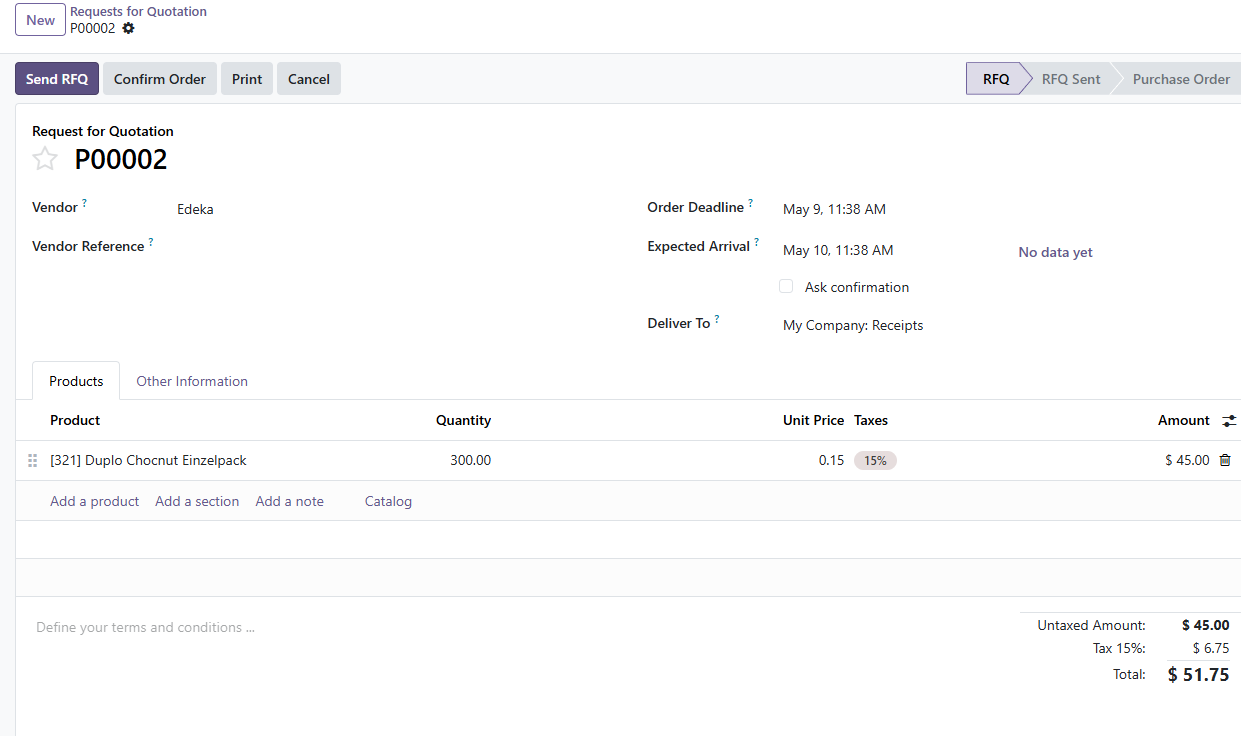
\includegraphics[width=0.95\textwidth]{Bestellung erzeugen.png}
    \figsource
    \label{fig:bestellung-erzeugen}
  \end{figure}

  \begin{figure}[htbp]
    \centering
    \caption{Bestätigung einer Bestellung}
    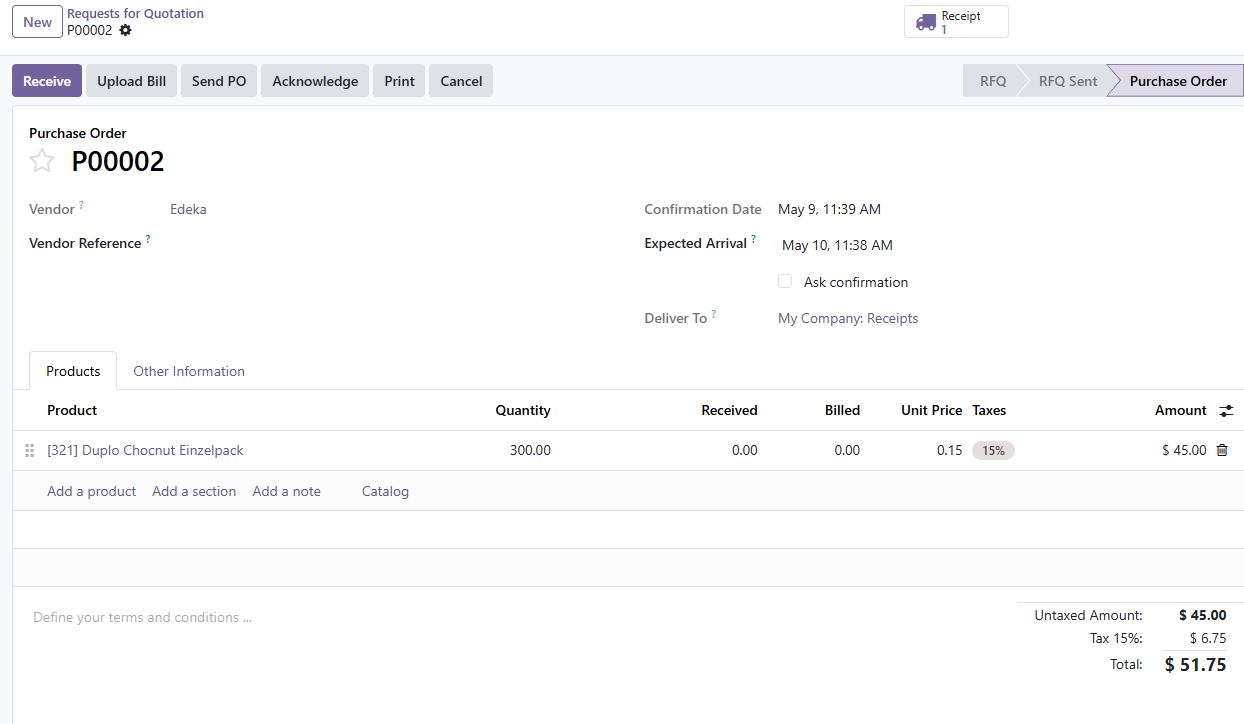
\includegraphics[width=0.95\textwidth]{Bestellung bestätigen.png}
    \figsource
    \label{fig:bestellung-bestaetigen}
  \end{figure}

  \begin{figure}[htbp]
    \centering
    \caption{Validierung einer Bestellung}
    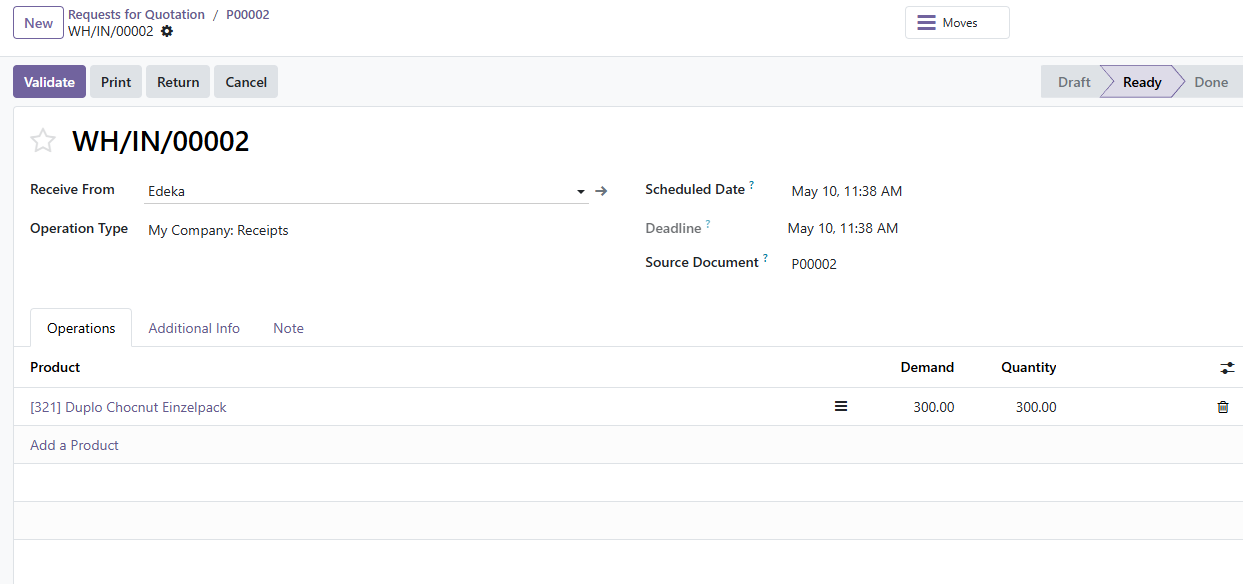
\includegraphics[width=0.95\textwidth]{Bestellung validieren.png}
    \figsource
    \label{fig:bestellung-validieren}
  \end{figure}

  \begin{figure}[htbp]
    \centering
    \caption{Abgeschlossene Bestellung im Beschaffungsprozess}
    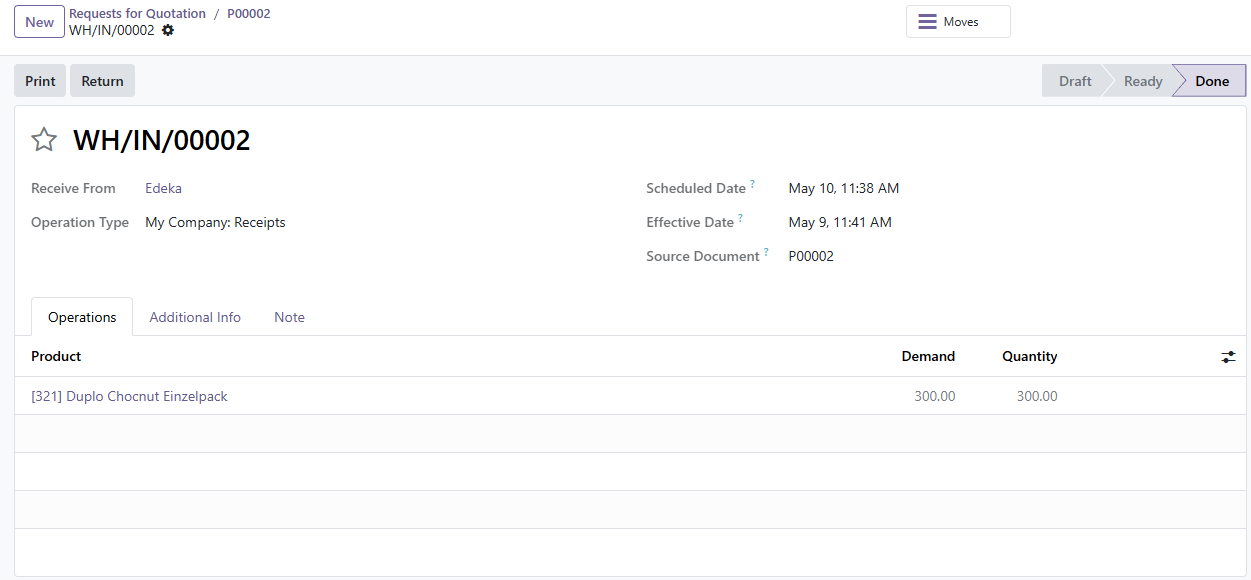
\includegraphics[width=0.95\textwidth]{Abgeschlossene Bestellung.png}
    \figsource
    \label{fig:abgeschlossene-bestellung}
  \end{figure}

\subsection{Erweiterung durch ein Custom-Submodul}

Für die prototypische Implementierung werden Python 3.12, Odoo 19 On-Premise, PostgreSQL ab Version 12 sowie ein Odoo-Custom-Addon für die API-Integration verwendet. Python dient dabei als Programmiersprache für die Geschäftslogik des Submoduls. Odoo stellt die ERP-Systemumgebung bereit, während PostgreSQL als relationale Datenbank für die Speicherung der ERP-Daten genutzt wird. Das Custom-Addon übernimmt die technische Verbindung zwischen Barcode-Eingabe, API-Abfrage und Produktdatenverarbeitung innerhalb von Odoo.

Die Erweiterung wird so konzipiert, dass die API-Integration nicht direkt im Odoo-Kernsystem umgesetzt wird, sondern in einer separaten Modullogik. Dadurch bleibt die Wartbarkeit der Lösung erhalten. Änderungen an der API-Verarbeitung, an Mapping-Regeln oder an Validierungsmechanismen können innerhalb des Custom-Submoduls vorgenommen werden, ohne die Standardmodule von Odoo unmittelbar zu verändern.

\section{Konzeption und Umsetzung des Barcode-API-Submoduls}

Dieses Kapitel beschreibt die Konzeption und technische Umsetzung des Submoduls. Der Schwerpunkt liegt auf dem Prozessablauf vom Barcode-Scan bis zum Produktdatensatz, der API-Integration und der Einbindung der erzeugten oder aktualisierten Produktdaten in Odoo.

\subsection{Prozessablauf vom Barcode-Scan bis zum Produktdatensatz}

Der Prozess beginnt mit der Erfassung eines Barcodes. Diese Erfassung kann über ein Barcode-fähiges Endgerät oder durch manuelle Eingabe erfolgen. Der Barcode wird anschließend vom Custom-Submodul entgegengenommen und als eindeutiges Identifikationsmerkmal für die weitere Verarbeitung genutzt. Im ersten Verarbeitungsschritt wird geprüft, ob in Odoo bereits ein Produktdatensatz mit diesem Barcode vorhanden ist. Diese Prüfung verhindert, dass identische Produkte mehrfach angelegt werden.

Ist bereits ein Produkt mit dem erfassten Barcode vorhanden, können bestehende Informationen aktualisiert oder ergänzt werden. Ist kein entsprechender Datensatz vorhanden, wird auf Grundlage der extern abgerufenen Produktinformationen ein neuer Produktstammsatz angelegt. Der Prozess umfasst somit das Empfangen des Barcodes, den Aufruf des Custom-Addons, die Abfrage der externen Datenquelle, die Verarbeitung der API-Antwort sowie das Erstellen oder Aktualisieren des Produktdatensatzes in Odoo.

Abbildung \ref{fig:barcode-import} zeigt die Erfassung des Barcodes im Importfenster, Abbildung \ref{fig:auto-produkt} die automatische Anlage des Produktdatensatzes nach der externen Datenanreicherung.

\begin{figure}[htbp]
  \centering
  \caption{Barcode-Importfenster im Prototyp}
  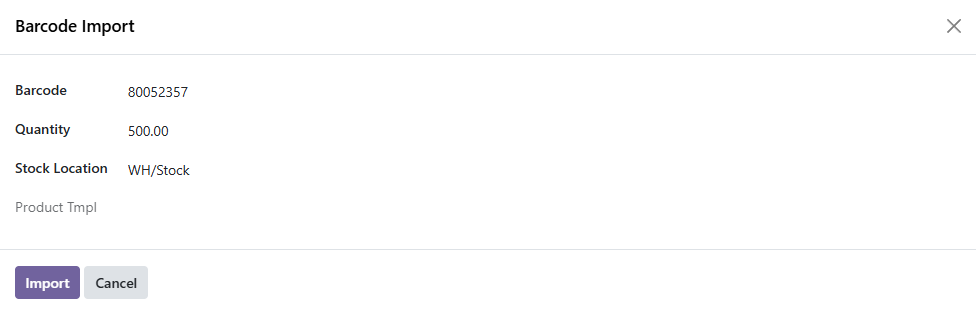
\includegraphics[width=0.95\textwidth]{Barcode Import Fenster.png}
  \figsource
  \label{fig:barcode-import}
\end{figure}

\begin{figure}[htbp]
  \centering
  \caption{Automatisch angelegtes Produkt nach der API-Verarbeitung}
  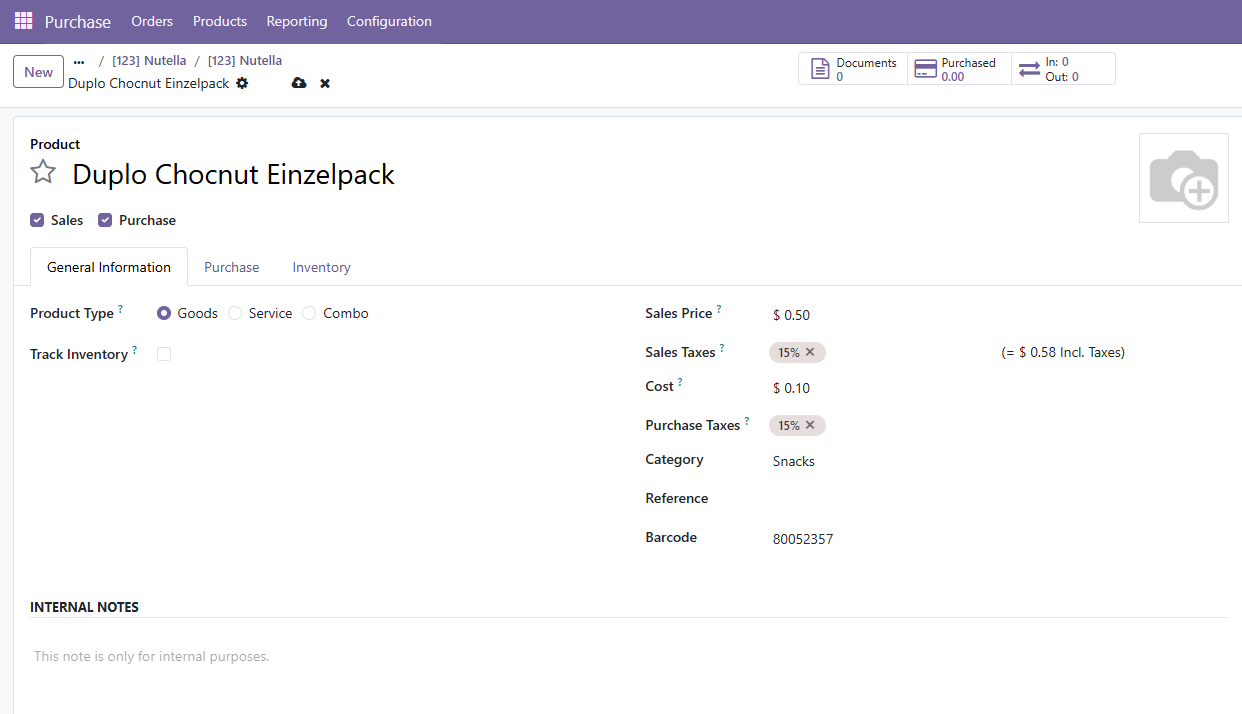
\includegraphics[width=0.95\textwidth]{Automatisch angelegtes Produkt.png}
  \figsource
  \label{fig:auto-produkt}
\end{figure}

\subsection{API-Abfrage und Datenübernahme aus Open Food Facts}

Die produktbezogene Datenabfrage erfolgt über einen Python-Service, der anhand des Barcodes eine Anfrage an die Open-Food-Facts-API sendet. Die Anfrage nutzt die Barcode-basierte Produktressource der API. Der technische Aufruf kann vereinfacht wie folgt dargestellt werden:

\begin{lstlisting}[caption={Produktbezogene API-Abfrage}, label={lst:product-api-request}]
GET /api/v0/product/{barcode}.json
\end{lstlisting}

Nach Eingang der API-Antwort werden die relevanten Datenfelder extrahiert und auf die entsprechenden Odoo-Modelle übertragen. Dazu gehören insbesondere Produktname, Hersteller- beziehungsweise Markeninformationen, Barcode sowie verfügbare Nährwert- und Produktinformationen. Die Datenübernahme erfolgt nicht ungeprüft, sondern muss berücksichtigen, dass externe Datensätze unvollständig sein können. Daher ist eine Verarbeitung erforderlich, die fehlende Felder erkennt und nur geeignete Informationen in die Produktverwaltung überführt.

Die übernommene Datenstruktur muss mit den Datenmodellen von Odoo kompatibel sein. Aus diesem Grund werden die aus der API erhaltenen Informationen in ein internes Mapping überführt. Dieses Mapping legt fest, welche API-Felder welchen Odoo-Feldern entsprechen. Auf dieser Grundlage können Produktdaten erstellt, aktualisiert und anschließend in nachgelagerten Prozessen verwendet werden.

\subsection{Integration in Lagerprozesse}

Sobald ein Produkt in Odoo vorhanden ist, kann es im Inventory-Modul verwendet werden. Dadurch wird es möglich, das Produkt in Wareneingängen zu verbuchen, Lagerbewegungen zu dokumentieren, Bestände zu verwalten oder das Produkt im Rahmen von Kommissionierungsprozessen auszulagern. Die automatische Produktanlage bildet damit die Grundlage für eine anschließende lagerbezogene Verarbeitung.

Die Integration in Lagerprozesse beruht darauf, dass Produktstammdaten und Lagerdaten im ERP-System miteinander verknüpft sind. Ein durch das Custom-Submodul angelegtes oder aktualisiertes Produkt kann dadurch denselben Prozessen zugeführt werden wie ein manuell angelegtes Produkt. Zusätzlich können die Produktdaten im Sales-Modul für Bestellungen und Verkaufsprozesse genutzt werden. Die Schnittstelle zwischen Barcode-Erfassung, externer Produktdatenquelle und Odoo-Produktmodell ermöglicht somit einen durchgängigen Prozess von der Produktidentifikation bis zur ERP-internen Weiterverarbeitung.

Die Abbildung \ref{fig:inventory-bestellfortschritt} dokumentiert den Bestellfortschritt im Inventory-Kontext; Abbildung \ref{fig:inventory-abgeschlossen} zeigt den abgeschlossenen Zustand nach der Verarbeitung.

\begin{figure}[htbp]
  \centering
  \caption{Inventory-Übersicht mit Bestellfortschritt}
  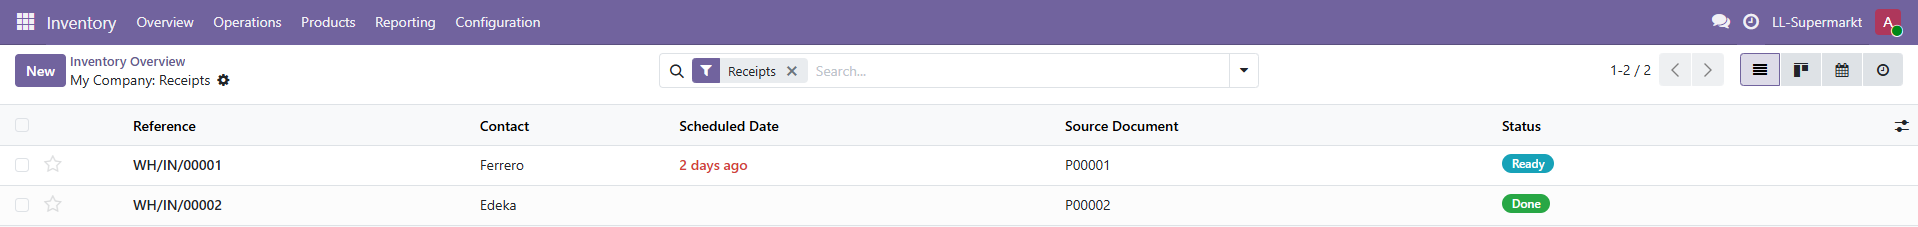
\includegraphics[width=0.95\textwidth]{Inventory Übersicht mit Bestellfortschritt.png}
  \figsource
  \label{fig:inventory-bestellfortschritt}
\end{figure}

\begin{figure}[htbp]
  \centering
  \caption{Abgeschlossene Bestellung im Inventory-Kontext}
  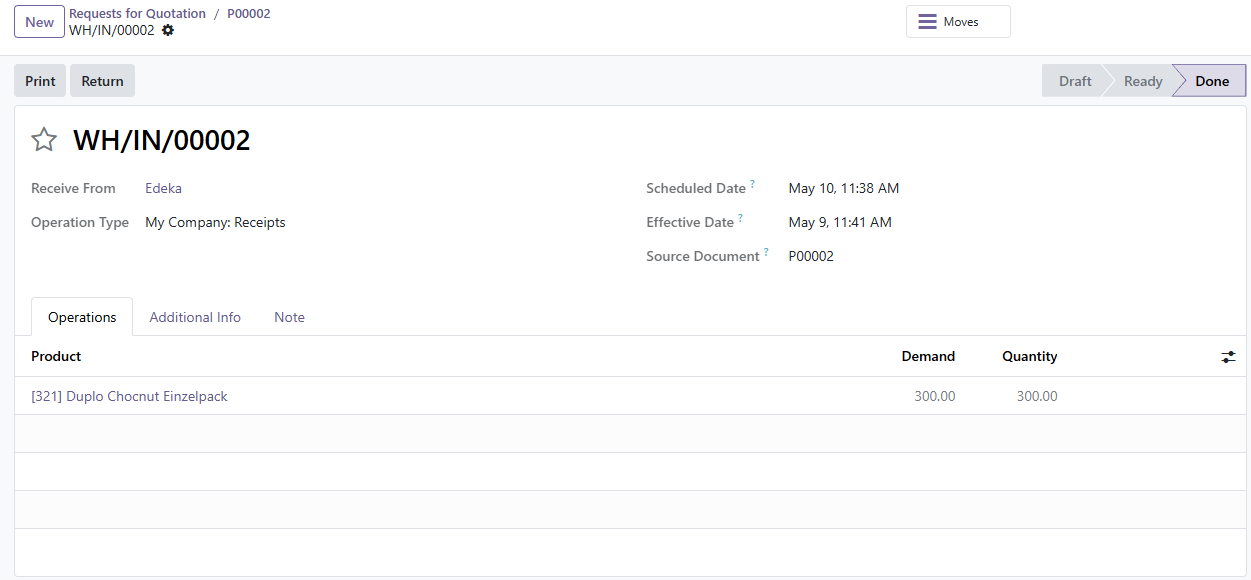
\includegraphics[width=0.95\textwidth]{Abgeschlossene Bestellung.png}
  \figsource
  \label{fig:inventory-abgeschlossen}
\end{figure}

\section{Analyse der Lösung}

\subsection{Vorteile gegenüber manueller Produktpflege}

Die entwickelte Lösung ersetzt Teile der manuellen Produktpflege durch einen API-gestützten Datenabruf. Der wesentliche Unterschied zur manuellen Vorgehensweise besteht darin, dass Produktinformationen nicht einzeln recherchiert und händisch in das ERP-System übertragen werden müssen, sofern sie über die Open-Food-Facts-API verfügbar sind. Stattdessen wird der Barcode als Schlüssel verwendet, um strukturierte Produktdaten aus einer externen Datenquelle abzurufen und in Odoo weiterzuverarbeiten.

Dadurch kann der manuelle Erfassungsaufwand bei der Produktanlage reduziert werden. Gleichzeitig wird die Wahrscheinlichkeit von Übertragungsfehlern verringert, da bereits strukturierte Daten übernommen werden können. Ein weiterer Vorteil besteht in der einheitlicheren Verarbeitung der Produktdaten, da die Zuordnung der API-Felder zu Odoo-Feldern über definierte Mapping-Regeln erfolgt. Die Lösung unterstützt somit eine systematische und reproduzierbare Pflege von Produktstammdaten.

Für Lager- und Verkaufsprozesse ist außerdem relevant, dass die Produktdaten unmittelbar nach ihrer Anlage im ERP-System verfügbar sind. Dadurch können sie in Wareneingängen, Bestandsbuchungen und Verkaufsprozessen weiterverwendet werden. Die Lösung stellt somit keinen isolierten Datenimport dar, sondern ist in die ERP-interne Prozesskette eingebunden.

\subsection{Grenzen, Fehlerfälle und Datenqualität}

Die prototypische Lösung ist von der Verfügbarkeit und Datenqualität der Open-Food-Facts-API abhängig. Nicht jeder Barcode ist in der Datenbank vorhanden. Zudem können vorhandene Datensätze unvollständig, uneinheitlich oder fehlerhaft gepflegt sein. In solchen Fällen können Produktinformationen nicht vollständig übernommen werden. Daraus ergibt sich die Notwendigkeit, API-Antworten zu prüfen und fehlende oder ungeeignete Datenfelder im Prozess zu berücksichtigen.

Ein weiterer Fehlerfall entsteht, wenn die API zeitweise nicht erreichbar ist oder keine gültige Antwort liefert. Das Submodul muss daher so gestaltet werden, dass ein fehlgeschlagener API-Aufruf nicht zu inkonsistenten Daten im ERP-System führt. Ebenso muss verhindert werden, dass Produkte mehrfach angelegt werden, wenn ein Barcode bereits im System vorhanden ist. Hierfür ist eine Prüfung bestehender Produktdatensätze erforderlich.

Die Datenqualität der externen Quelle kann durch das ERP-System nicht vollständig kontrolliert werden. Das Custom-Submodul kann lediglich Regeln für die Übernahme, Validierung und Weiterverarbeitung der gelieferten Daten bereitstellen. Daraus folgt, dass die automatisierte Stammdatenpflege nicht als vollständiger Ersatz für Datenqualitätsmanagement verstanden werden kann. Vielmehr stellt sie eine technische Unterstützung dar, die manuelle Prozessschritte reduziert und die strukturierte Übernahme externer Produktinformationen ermöglicht.

\section{Fazit und Ausblick}

Die Arbeit zeigt, dass eine automatisierte Stammdatenpflege im ERP-System Odoo durch Barcode-Erfassung und API-Integration technisch umsetzbar ist. Der entwickelte Prototyp verbindet die Eingabe oder den Scan eines Barcodes mit einer externen Produktdatenabfrage über die Open-Food-Facts-API und der anschließenden Erstellung oder Aktualisierung eines Produktdatensatzes in Odoo. Dadurch wird ein durchgängiger Prozess von der Produktidentifikation bis zur ERP-internen Weiterverarbeitung abgebildet.

Es wurde dargestellt, dass die Lösung insbesondere für die Reduktion manueller Erfassungsschritte geeignet ist, sofern die benötigten Produktdaten in der externen Datenquelle vorhanden und ausreichend vollständig sind. Die Daten können nach der Übernahme in Odoo für Lagerprozesse im Inventory-Modul und für nachgelagerte Verkaufsprozesse im Sales-Modul genutzt werden. Gleichzeitig wurde deutlich, dass die Qualität der automatisierten Produktanlage von der Verfügbarkeit und Vollständigkeit der Open-Food-Facts-Daten abhängt.

Für zukünftige Arbeiten ergeben sich mehrere Erweiterungsmöglichkeiten. Zum einen könnten zusätzliche Produktdatenquellen integriert werden, um die Abhängigkeit von einer einzelnen externen Datenbank zu reduzieren. Zum anderen könnten erweiterte Validierungsregeln ergänzt werden, um unvollständige oder widersprüchliche API-Antworten systematischer zu behandeln. Darüber hinaus wäre eine mobile-first-orientierte Umsetzung denkbar, bei der Barcode-Erfassung, Produktdatenabfrage und Lagerbuchung stärker auf mobile Endgeräte ausgerichtet werden. Auch die Ergänzung bildbasierter Analysen könnte geprüft werden, sofern Produktbilder oder Verpackungsinformationen automatisiert ausgewertet werden sollen.


% ---------------------------------------------------
% CODEVERZEICHNIS
% ---------------------------------------------------
\newpage
\phantomsection
\addcontentsline{toc}{section}{Codeverzeichnis}
\lstlistoflistings

% ---------------------------------------------------
% LITERATURVERZEICHNIS
% ---------------------------------------------------
\newpage
\printbibliography[heading=bibintoc, title={Literaturverzeichnis}]

% ---------------------------------------------------
% KI-HILFSMITTELVERZEICHNIS
% ---------------------------------------------------
\newpage
\section*{KI-Hilfsmittelverzeichnis}
\addcontentsline{toc}{section}{KI-Hilfsmittelverzeichnis}

\begin{tabular}{@{}p{1cm}p{4cm}p{9.5cm}@{}}
\toprule
\textbf{Nr.} & \textbf{KI-System} & \textbf{Einsatzzweck} \\ 
\midrule
1 & Google Gemini, Version X.X, Zugriff am TT.MM.JJJJ & Unterstützung bei der Formulierung von Textentwürfen zur Einleitung und zu konzeptionellen Grundlagen. Die übernommenen Inhalte wurden fachlich geprüft und überarbeitet. \\
2 & ChatGPT & Unterstützung bei der formalen Strukturierung der LaTeX-Vorlage nach dem FOM-Leitfaden. \\
\bottomrule
3 & ChatGPT & Vervollständige das Abkürzungsverzeichnis \\
4 & ChatGPT & Schreibe stichpunkte zu diesen kapiteln, auf basis des programmierten moduls:
4 Konzeption und Umsetzung des Barcode-API-Submoduls 4.1 Anforderungen an das Submodul 4.2 Prozessablauf vom Barcode-Scan bis zum Produktdatensatz 4.3 API-Abfrage und Datenübernahme aus Open Food Facts 4.4 Automatische Produktanlage in Odoo 4.5 Integration in Lagerprozesse

\end{tabular} 

\end{document}